\documentclass[10pt]{article}
\usepackage{amsmath,amssymb,graphicx}
\usepackage{hyperref}
\setlength\parindent{0pt}
\begin{document}
\title{Assignment 1: Sparse Matrices}
\author{1212550}

\section{The Gauss Seidel Algorithm}
The  $\textit{Gauss Seidel}$  algorithm is a Splitting method used to solve a system of linear equations, which we represent in matrix form as $Ax=b$. A Splitting method has the general form
\[ Px^{(k+1)} = Nx^{(k)} + b, \]
where $A = P - N$ is the matrix splitting. This is equivalent to
\[ x^{(k+1)} = x^{(k)} + P^{-1}r^{(k)}, \]
where $r^{(k)} = b - Ax^{(k)}$ is called the residual. For the implementation of this method we redifine our decomposition of $A$ to be $A = D - (E+F)$, where $-E,D,-F$ are the lower triangular matrix, diagonal matrix and upper triangular matrix of $A$ respectively. For the $\textit{Gauss Seidel}$ method itself, $P = D - E$ and $N = F$. The convergence of iterations of this type depends on the spectral radius $\rho(P^{-1}N)$, where
\[ \rho(A) = \text{max}\{ |\lambda|: \lambda \in \lambda(A) \}. \]
The $\textit{Gauss Seidel}$ method can be applied to any matrix with non-zero elements on the diagonals, but convergence is only guaranteed if the matrix is either diagonally dominant, or symmetric and positive definite. \\

Noting that the matrix $P$ is in triangular form, and
\[ x^{(k+1)} = P^{-1}(Nx^{(k)} + b),\]
the elements $x^{(k+1)}$ can be computed using forward substitution. Thus it follows that
\[ x_i^{(k+1)} = \frac{1}{a_{ii}} \Big( b_i - \sum_{j=1}^{i-1}x^{(k+1)}a_{ij} - \sum_{j=i+1}^{n}x^{(k)}a_{ij} \Big), \]
for $i = 1,...,n$. The procedure continues until the residual error, defined by $||r^{(k)}|| = ||b- A x^{(k)}||$, is below some tolerance or the algorithm has stagnated. For the implementation used in this assignment, the norm is the $L^{\infty}$-norm. Note that elements of the approximation $x^{(k)}$ can be overwritten in this algorithm, so only one storage vector for the approximation will be needed in practice. \\

For this assignment I have implemented a $\textit{SparseMatrix}$ class, which stores matrices in row major format in such a way that only non-zero elements are stored in memory. It contains a member function which allows the user to add entries to a blank matrix of their choice dimensions, along with other useful functions. In particular, it has a member function called $\textit{GaussSeidel}$, which, for an initial guess $x^{(0)}$ and input vector $b$, performs the above algorithm and returns a vector containing the residual error for each iteration. This will implicitly return the number of iterations computed, since it will be equal to the size of the vector.\\

I have set the function such that it continues iterating as long as the residual error for each iteration is above a tolerance of $1e - 6$ and no more than $100,000$ iterations have been computed. Furthermore, the function checks that the input vectors are of appropriate dimension and that the diagonal of the matrix is non-zero. If any of these errors occur, the returned vector contains the residual error between $b$ and $x^{(0)}$ only. A warning stating this is issued to the user in these cases.

\section{Testing the Algorithm}
I have tested my implementation for matrix $A \in \mathbb{R}^{N \times N}$ and vector $b \in \mathbb{R}^N$ defined as follows for $i,j = 0,...,N-1$:

$$a_{ij}=
\begin{cases}
-D_i &\text{for} \quad j = i-1\\
D_i + D_{i-1} &\text{for} \quad j=i\\
-D_{i} &\text{for} \quad j = i + 1\\
0 &\text{otherwise}
\end{cases}
$$
where $D_i=a(w_i - \frac{1}{2})^2 + \delta$, $w_i = \frac{i+1}{N+1}$ for constants $a=(4-\delta)$, $\delta > 0$, and
$$b_{i}=
\begin{cases}
-2a(w_i - \frac{1}{2})w_0^2 &\text{for} \quad i = 0,...,N-2\\
-2a(w_i - \frac{1}{2})w_0^2 + 1 &\text{for} \quad i=N-1.
\end{cases}
$$
Initially $\delta$ was set to be $1$, and the method was tested for $N=100$, $1000$, and $100000$.

Here are some results. The function is approximated on a grid with
$N=128$ gripoints. See figure~\ref{fig:func_and_deriv} for results.
 \begin{figure}%
 \begin{center}
    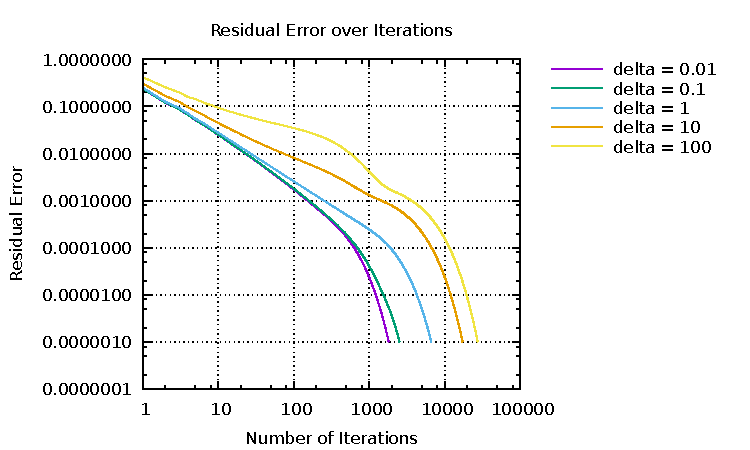
\includegraphics[width=0.49\textwidth]{function}
    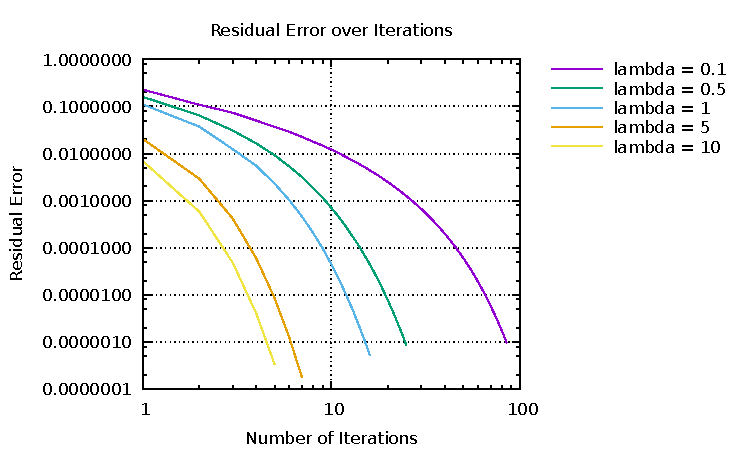
\includegraphics[width=0.49\textwidth]{function2}
  \end{center}
  \caption{This is the figure. Left: Function $f(x)=\sin(x)$. Right:
    Derivative $f'(x) = \cos(x)$. Note that the $x$-axis shows
    gridpoint-indices and not the proper $x$ value.
  \label{fig:func_and_deriv}}
\end{figure}

\end{document}
